\documentclass{article}
\usepackage[utf8]{inputenc}
\usepackage[pdftex]{graphicx}
\usepackage{gensymb}
\usepackage[letterpaper, margin=1in]{geometry}
\usepackage{setspace}
\onehalfspacing


\begin{document}

\begin{titlepage}
    \begin{center}
        \vspace*{1cm}
 
        \Huge
        \textbf{Real Estate Investment Opportunities in the GTA}
 
        \vspace{0.5cm}
        \LARGE
        Capstone Report
 
        \vspace{1.5cm}
 
        \textbf{Jonathan Densil}
 
        \vfill
 
 
        \vspace{0.8cm}
 
        
\includegraphics[width=0.4\textwidth]{ibm.png}
        
        \Large
        IBM Data Science Professional Certificate\\
        Coursera Inc.\\
        \today
 
    \end{center}
\end{titlepage}

\section{Introduction}

The Greater Toronto Area (GTA) is the most populous metropolitan area housing around 20\% of the population of Canada. Serving as the anchor of the GTA, the second-largest financial sector in North America. Toronto is the 4\textsuperscript{th} largest city in North America and Canada's business and financial capital. The GTA also has nearly 100,000 new immigrants annually and 130 million people within a 500 mile radius; such a large flux of people would provide ample real estate investment opportunities.   

\begin{figure}[h]
	\centering
	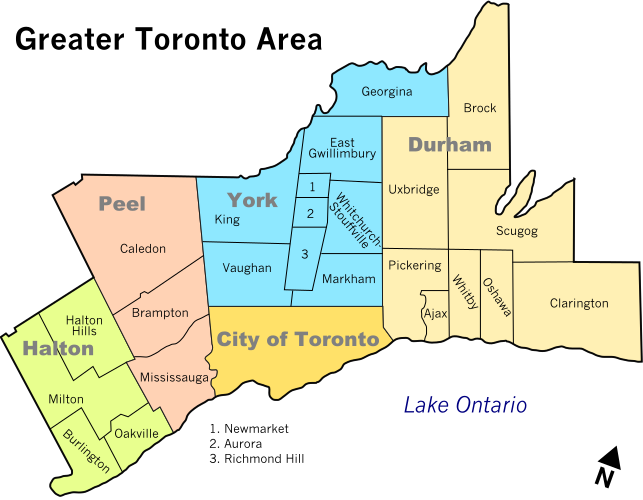
\includegraphics[width=\textwidth]{gta_map.png}
	\caption{Municipalities in the GTA}
	\label{gta}
\end{figure}


\section{Business Problem}

As the old adage goes: location, location, location. Using machine learning and artificial intelligence to determine the best locations to buy a home or commercial real estate will be a key tool for realtors in advising clients of where to invest. Developing this kind of model would also be of great value to immigrants and internal migrants seeking to buy a home in an new and unknown location, giving them a sense for the community before committing to a life-changing decision.


\section{Data}

In order to create the dataset needed to train the machine learning algorithm, we will need the following data:

\begin{itemize}
	\item Real estate sales in Ontario to determine a range of affordability options
	\item Popular venues and attractions that will potentially raise the house prices and attract traffic
	\item Geolocation data to visualise the potential areas of interest  
\end{itemize}

Housing sales data was taken from a kaggle dataset (https://www.kaggle.com/mnabaee/ontarioproperties) since the Canadian Real Estate Association (CREA) prohibits the publication of any analyses, graphs, charts, results, conclusions or forecasts of the MLS\textsuperscript{\textregistered} House Price Index (HPI) data without the prior written consent of CREA. Geolocation location was taken from the Atlas of Canada and popular venue data was queried using the Foursquare API. 

\end{document}

